\section{An exact variational calculation on an interval}
\label{sec:var}

What is the least possible uniform error when approximating $x^2$ on $[0,1]$ by a $[0,1]$-valued $L$-Lipschitz function? This is a closed expression of the preceding language:
\[
 V(L)=\inf_{f\in\Lip_L([0,1],[0,1])}\ \sup_{x\in[0,1]}|f(x)-x^2|.
\]
The inner observable is uniformly continuous in both inputs, since squaring is $2$-Lipschitz on $[0,1]$. Its supremum remains $1$-Lipschitz in $f$. Finite nets therefore compute a regular name for $V(L)$. In this case one can do better and find an optimal function.

\begin{theorem}[Sharp Lipschitz approximation of a square]\label{thm:minimax}
For rational $L\ge0$ put $t=\min(1,L/2)$ and $E=(1-t)^2/2$. Then
\[
 V(L)=E=\frac{(\max(0,2-L))^2}{8},\qquad
 g(x)=E+x^2-(\max(0,x-t))^2
\]
attains this value. The rational formula gives a PR name for $g$ uniformly in $L$. The value formula also extends to named nonnegative slopes by its displayed continuous expression.
\end{theorem}
\begin{proof}
First suppose $0\le L\le2$, hence $L=2t$. If $\|f-x^2\|_\infty\le e$, then
\[
 1-e\le f(1)\le f(t)+2t(1-t)\le t^2+e+2t(1-t).
\]
Rearranging yields $2e\ge(1-t)^2$. This uses only the two evaluations $1,t$. Equivalently the actual supremum error of each $f$ bounds $E$, by Lemma~\ref{lem:sup}.

For the upper bound the proposed function equals $E+x^2$ on $[0,t]$ and $E+2tx-t^2$ on $[t,1]$. Both formulas agree at $t$. For $x\le y\le t$, its increment is $(y-x)(y+x)$, between $0$ and $2t(y-x)$. On $[t,1]$ the increment equals $2t(y-x)$. Across $t$, add the two bounds. Thus $g$ is nondecreasing and $2t$-Lipschitz. Its endpoint values are $E$ and $1-E$, both in $[0,1]$. Its signed error $g(x)-x^2$ equals $E-(\max(0,x-t))^2$, which ranges between $E$ and $-E$ and attains both bounds (they coincide when $t=1$). For $L\ge2$ the original square is already $L$-Lipschitz, $t=1$ and $E=0$. The case $L=0$ gives the constant $1/2$ as a check.

The case distinctions apply to rational observations. For a completed input evaluate the single maximum formula and use the preceding Lipschitz bound on the dense rationals. Products of bounded numbers and rational min/max have explicit moduli. For example on $[0,1]$, changing both arguments of $x^2-(x-t)_+^2$ by at most $\epsilon$ changes the expression by at most $6\epsilon$ by difference of squares, and $E$ changes by at most $\epsilon$. Thus one fixed precision shift also computes values jointly in $x,t$. The closed value formula in $L$ is continuous at the breakpoint. The arithmetic lower bound for each fixed family $f$ with an $L$-Lipschitz contract is an inequality of names obtained by two evaluations and removal of finite rational slack. The upper bound provides the algorithm $g$ and proves its contract.
\end{proof}

\begin{figure}[htbp]
\centering
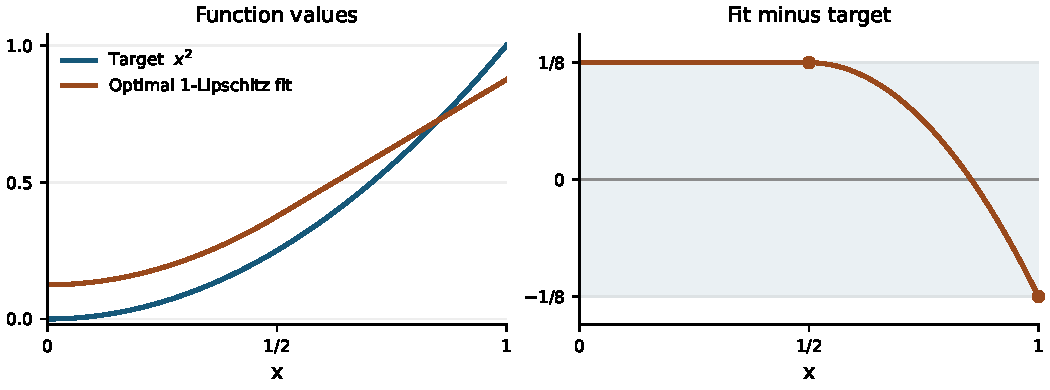
\includegraphics[width=.91\linewidth]{figures/variational.pdf}
\caption{At $L=1$, the optimal function meets its two extremal signed errors at $x=1/2$ and $x=1$. Those two evaluations already force the error $1/8$.}
\end{figure}

The finite-data analogue explains how the lower bound can be found. Suppose $u_i\in[0,1]\cap\Q$ are prescribed at a nonempty finite list of anchors $a_i\in D$. Put
\[
 e_*=\tfrac12\max_{i,j}\bigl(|u_i-u_j|-Ld(a_i,a_j)\bigr)_+.
\]
A fit of error $e$ at all anchors implies $|u_i-u_j|\le 2e+Ld(a_i,a_j)$, so $e\ge e_*$. To attain it, take the minimum of $1$ and the cones with heights $u_j+e_*$. Heights above one may be clipped to one, since their cones never lower that capped minimum. At $a_i$ the $i$-th cone gives the upper bound $u_i+e_*$. For every $j$, $u_j+e_*+Ld(a_i,a_j)\ge u_i-e_*$, and the cap is also at least $u_i-e_*$. Hence the error is at most $e_*$ and Lemma~\ref{lem:anchors} proves feasibility. Repeated anchor positions are allowed. This certificate explains why two opposed sample constraints determine the lower bound in the continuous example.

The file \texttt{Variational.lean} checks the rational lower bound, feasibility and attainment for arbitrary rational $0\le t\le1$ and every candidate $f:\Q\to\Q$ satisfying the interval guards. For real-valued named $f$ the lower-bound proof above uses the same rational inequalities with independent evaluation slack. The Lean quantifier over $f$ belongs to the metatheory. The object-language endpoint quantifies only over numerical parameters of a prescribed evaluator and its rational sample precision.

\subsection{An optimization over functionals}

There is a categorical reason the same answer survives a change of domain. Suppose $r:Y\to X$ and $s:X\to Y$ are nonexpansive maps with $r(s(x))=x$, and $u:X\to[0,1]$ is uniformly continuous. Call $e\ge0$ attainable if some $L$-Lipschitz $g:X\to[0,1]$ fits $u$ to uniform error at most $e$. Exactly the same tolerances are attainable on $Y$ for $u\circ r$. Indeed $g\circ r$ supplies the forward witness. For the converse, if $h$ fits $u\circ r$ on $Y$, the function $h\circ s$ fits $u$ on $X$ with the same error. Both composites preserve the Lipschitz constant. Whenever the infima are presented by our nets, these two witness transformations also give equal infima: apply them to the finite near-minimizers and let their prescribed errors decrease. An optimal witness on $X$ pulls back to an optimal witness on $Y$. Nonexpansiveness of both arrows controls the Lipschitz constant in these two transformations. The Lean theorem \texttt{fits\_retract} checks the witness equivalence on rational pseudometric carriers.

For an example in which the unknown is a functional, take $Y=\Lip_1([0,1],[0,1])$, $r(f)=f(1/2)$, and let $s(a)$ be the constant function $a$. Evaluation is nonexpansive in $f$; the uniform distance between two constant functions is exactly the distance of their values. The identity $r\circ s=\mathrm{id}$ is pointwise evaluation. Consequently
\[
 \inf_{\Phi\in\Lip_L(Y,[0,1])}\ \sup_{f\in Y}
       |\Phi(f)-f(1/2)^2|=\frac{(\max(0,2-L))^2}{8}.
\]
An optimal functional is $\Phi(f)=g(f(1/2))$ with $g$ from Theorem~\ref{thm:minimax}. All the constructions have algorithms on names: $r$ evaluates a cone name at the rational midpoint, while $s$ reads the scalar at the height precision and uses Theorem~\ref{thm:inner} to produce codes for the constant function. A single finite code need not encode an arbitrary constant exactly. On the lower-bound side only the constant functions of values $t$ and $1$ are needed. Thus the same two witnesses give the sharp answer even after two successive function-space constructions.
